\section{Introduction}

%q1: tale 1 of different level. but the setup is in exp. q2: cka vs cca. from high level why cka does not work. say from ns. when 1d in ns, svcca is same as pearson. need to check








% what make llm intelligent? An invest into stuctu property of atten heads.

% chara of a more intelligent llm. 
% llm has great ability, even close to human. we do not know what llm is a smarter one. to get smarter llm, we do not have a guidance. this is the goal.


% considering the close of human brain and llm, in ns xxx. 
% cv network has 
% inspired from ns, 
% goal: info smarter llm

% we compare llm and brain. inspired by ns, we study xxx. we focus on swi, and its correlation w.r.t intelligence. we find it is same as human brain. indicates that llm' head activation. based on the finding. prune can add to 2-3 sentences. pruneing to preserve the swi metric. this verify the impact of the metrics.




% figure, draw multiple layers
% change the circle to different color, give path a line

% change figure 1 to two figures
% make swi-perf with real data
% stack the two figures.


% prelim: 1. define swi. different quantity. how it used in ns, and the conclusion in ns.
% 2. notation

% key insights have a new section. 1. show how the graph is built (what data is used, what factor is tested by the data) 
% 2. and the exp results. 

% application driven by our finding: say two scores and used in pruning.
% goal: maintain swi. as considering pruning, global compute has issue. rather than comuting, we define xxx scores. potentially preserve swi. they can support head/layer.
% ADD!!!! core/bridge score illustration

% exp: 1. prove scors can preserve swi. ADD LLAMA.
% 2. pruning model results
% 3. intelli results
% 4. abl


% Large language models (LLMs) have demonstrated increasingly strong reasoning abilities, approaching human-level performance on a growing range of benchmarks \cite{leon2025gpt, liu2025deepseek, gardinazzi2024persistent}. Understanding why some models reason better than others is therefore central to explaining and improving model intelligence. Benchmarks help measure this difference by evaluating model behavior across diverse reasoning tasks \cite{wang2024mmlu, kaplan2020scaling, schaeffer2023emergent}. Moving from measurement to explanation requires identifying the internal organization that give rise to stronger reasoning ability \cite{liang2022holistic, rai2024practical}. This motivates a central question: what structural properties distinguish more capable LLMs from less capable ones?

Large language models (LLMs) have demonstrated increasingly strong reasoning abilities, approaching human-level performance on a growing range of benchmarks \cite{leon2025gpt, liu2025deepseek, gardinazzi2024persistent}. Existing benchmarks measure these abilities by evaluating model behavior across diverse reasoning tasks \cite{wang2024mmlu, kaplan2020scaling, schaeffer2023emergent}. However, behavioral evaluation alone does not explain why some models reason better than others. To move from measuring reasoning performance to understanding its underlying mechanisms, we need to examine how reasoning capability is encoded in the model itself. In particular, the neural activation
%\yy{you said neural activations are more accurate?} 
of an LLM may exhibit structural properties that reflect how the model organizes and composes information for reasoning \cite{zhang2024interpreting, rai2024practical}. This motivates a central question: what structural properties of internal organization distinguish more capable LLMs from less capable ones?
%on fluid intelligence benchmarks, which emphasize abstract reasoning and rule generalization \cite{yang2025truly, wu2025understanding}?



Existing structural analyses provide useful starting points. You et al. model neural architectures as relational graphs, where nodes denote computational units and edges encode message-passing connectivity, and show that architecture-level topology is predictive of generalization performance in computer vision models \cite{you2020graph}. However, this graph representation is determined by the architecture itself and is therefore largely independent of the training data and optimization process. Since reasoning ability is shaped by data-dependent training and can vary across models with similar architectures, architecture-level topology alone cannot explain why some trained LLMs reason better than others. Moreover, these analyses have primarily been applied to vision models, leaving open how to characterize the internal organization of trained LLMs.
% However, because this graph representation is specified by the network architecture rather than inferred from learned, data-dependent model behavior\yy{just say it is irrelevant to the training data and the optimization process, thus cannot be used to measure the reasoning abilities of the LLMs which is data- and training- dependent. also mention they only apply to vision models, not LLMs}, it does not capture the organization that emerges in a particular trained model. 
Another line of work studies trained models through the spectra of their learned weight matrices. Grounded in random matrix theory and Heavy-Tailed Self-Regularization Theory \cite{hu2025eigenspectrum, lu2024alphapruning}, these methods analyze empirical spectral densities and shape metrics, such as spectral decay and heavy-tailed behavior, to characterize training quality, generalization behavior, and pruning sensitivity~\cite{martin2021predicting, yang2023test}.
These spectral methods suggest that internal structure is informative, but they leave open whether it is associated with intelligence-related reasoning performance and provide limited insight into structural organization.
% These spectral methods suggest that internal structure is informative, but they leave open whether such structure associated with intelligence-related reasoning performance and provide limited insights on structural organization.
% \yy{you can also mention they are spectral methods, providing limited insights on structural organization and development of methods for structural intervention} 
To investigate the functional organization of LLMs, we draw inspiration from neuroscience, where intelligence has been linked to the topology and efficiency of functional brain networks \cite{langer2012functional, barbey2018network}. Functional brain networks treat anatomical regions of interest (ROIs) as nodes and define edges by statistical dependencies computed over their activity time series, rather than by anatomical connectivity alone. Prior studies have linked intelligence-related performance to functional brain network efficiency, often characterized by small-world properties such as high clustering coefficient and short path length \cite{langer2012functional, rosenberg2020functional}. Such organization is thought to support efficient information processing by combining densely connected local neighborhoods with short communication paths between distant regions \cite{latora2001efficient, bassett2017small}. Motivated by these findings, we ask whether activations in LLMs reveal analogous graph signatures associated with intelligence-related reasoning performance.


% Spectral properties of weight matrices have been linked to trained model quality \cite{hu2025eigenspectrum, lu2024alphapruning}, and graph-based analyses show that architectural connectivity can influence the predictive performance of deep neural networks \cite{you2020graph}.
% However, these studies mainly characterize weight statistics or architectural connectivity, and do not directly explain what internal structures distinguish LLMs that perform better on intelligence-related reasoning tasks.
% To seek such principles, we turn to neuroscience, where intelligence has been linked to the organization of functional brain networks \cite{langer2012functional, barbey2018network}. 
% In particular, higher intelligence-test performance has been associated with stronger small-world organization, reflected by higher local clustering and shorter characteristic path lengths \cite{langer2012functional, rosenberg2020functional}. 
% This topology supports efficient information processing through dense local connectivity and short communication paths across distant brain regions \cite{latora2001efficient, bassett2017small}. 
% This raises a natural question: do LLMs exhibit analogous internal structures that relate to their intelligence?


% \yy{Prior work has begun to study model capability through the lens of internal structure. You et al. model neural architectures as relational graphs, where nodes denote computational units and edges encode message-passing connectivity, and show that architecture-level topology is predictive of generalization performance in computer vision models \cite{you2020graph}. However, because their graph representation is determined by the network architecture rather than learned from data and optimization, it does not capture training- and data-dependent properties of a particular model. Moreover, their analysis focuses on vision models, leaving open how to characterize graph structure in the learned weights of LLMs and how such structure relates to reasoning ability. A complementary line of work studies trained models through the spectra of their learned weight matrices. Grounded in random matrix theory and Heavy-Tailed Self-Regularization, these methods analyze empirical spectral densities and associated shape metrics, such as spectral decay and heavy-tailed behavior, and relate them to model quality, training state, generalization, or pruning sensitivity \cite{hu2025eigenspectrum, lu2024alphapruning}. [cite a 2 more works here] While this line of work shows that learned weights contain informative signatures of trained models, it characterizes weights primarily through spectral matrix statistics. In contrast, we ask whether learned LLM weights exhibit graph organization that is associated with intelligence-related reasoning performance. }

% \yy{To guide the search for such organization, we draw inspiration from neuroscience, where intelligence has been linked to the topology and efficiency of functional brain networks \cite{langer2012functional, barbey2018network}. Functional brain networks represent brain regions as nodes and functional interactions, typically estimated from statistical dependencies in neural activity, as edges. Prior studies have linked intelligence-related performance to functional brain network efficiency, often characterized through small-world properties such as high clustering coefficient and short path length \cite{langer2012functional, rosenberg2020functional}. Such organization is thought to support efficient information processing by combining densely connected local neighborhoods with short communication paths between distant regions \cite{latora2001efficient, bassett2017small}. Motivated by these findings, we ask whether graph signatures in learned LLM weights are also associated with their reasoning capability.}


\begin{figure}%{r}{0.58\textwidth}
    \centering
    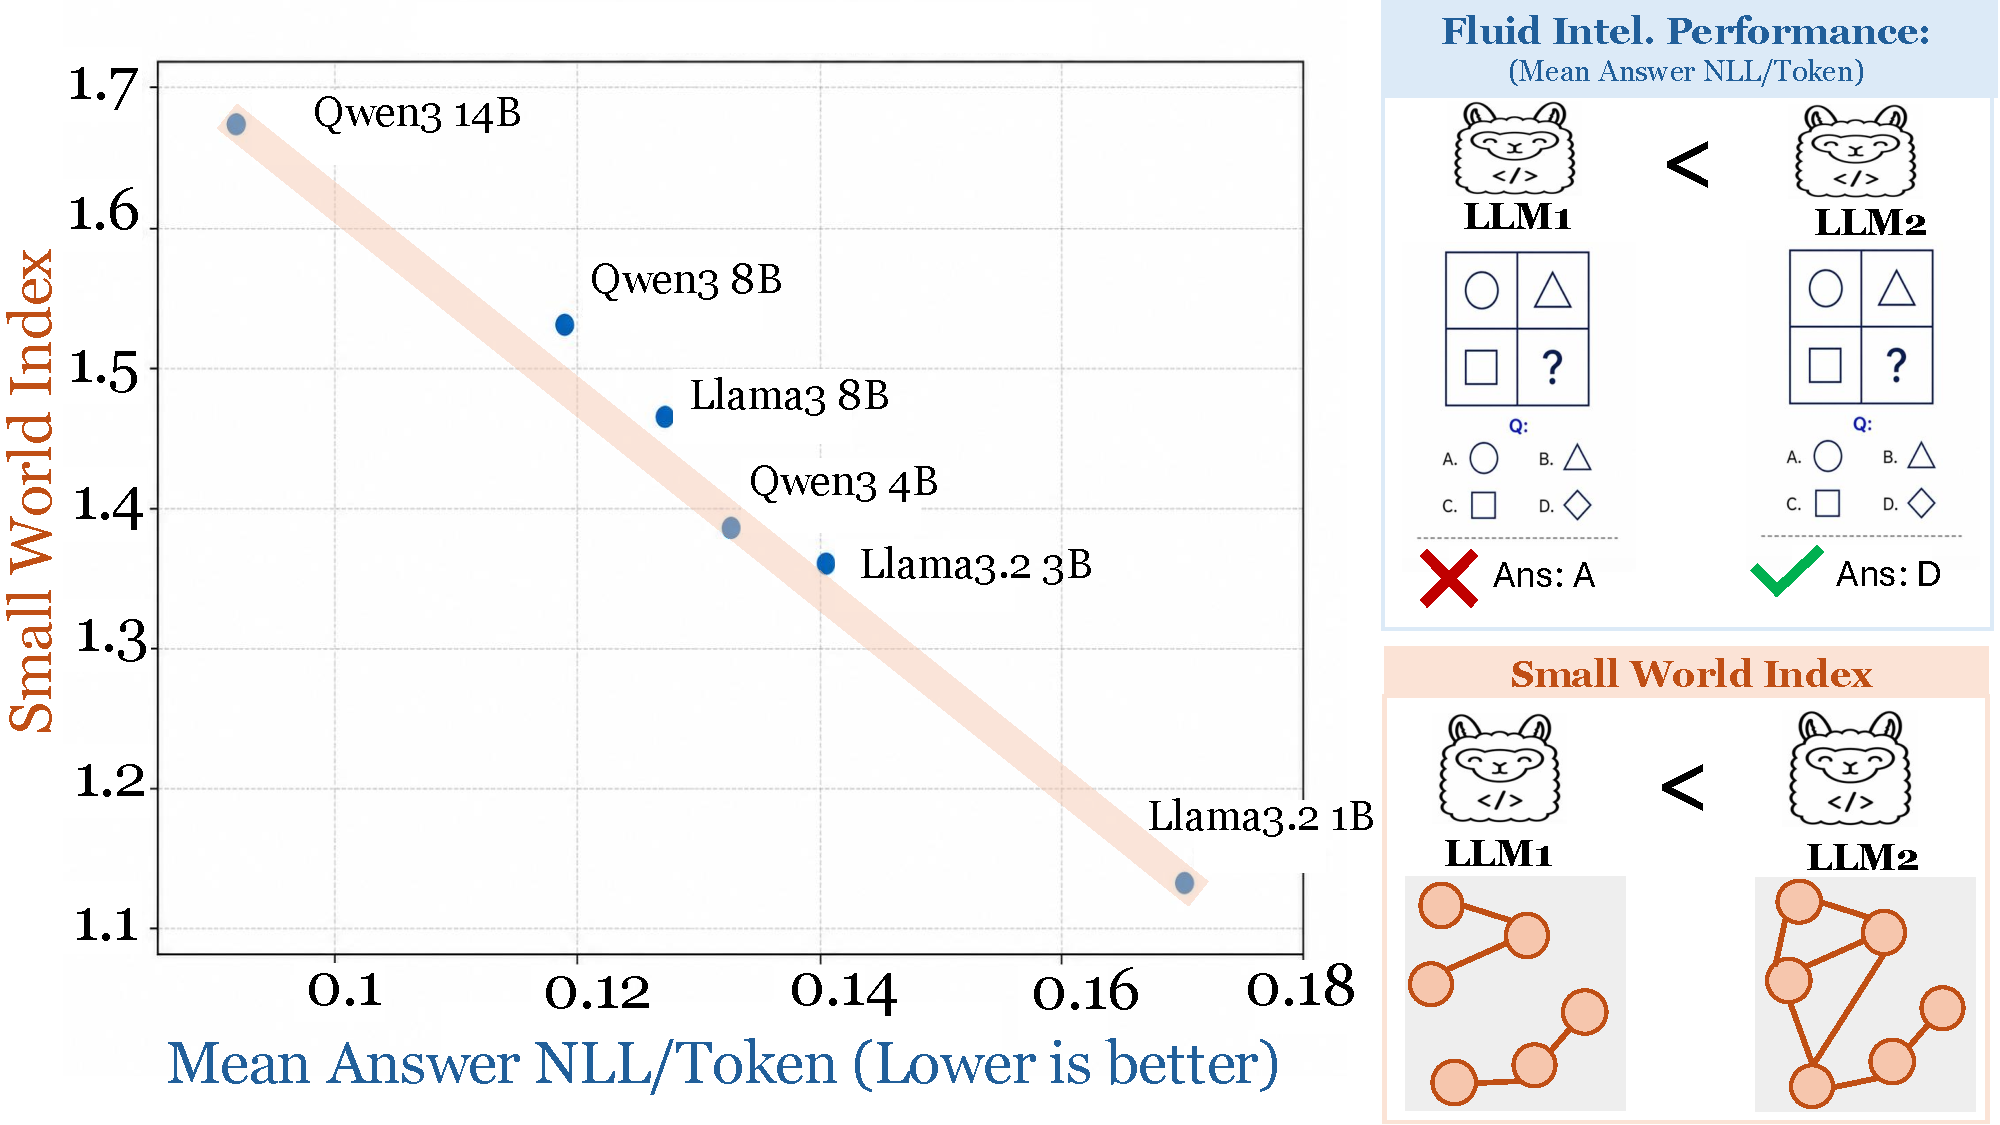
\includegraphics[width=\linewidth]{figure/swi-perf.pdf}
    \caption{\small Across LLMs, a higher small-world index (SWI; y-axis) is consistently associated with better fluid reasoning performance, measured by lower negative log-likelihood (NLL) per answer token on DRE-Bench \cite{yang2025truly} (x-axis).}
    \label{fig:swi-perf}
\end{figure}


In this work, we answer this question by studying the functional organization of LLMs. We focus on attention heads and construct a functional graph in which nodes represent heads and edges are defined by activation similarity. By measuring the small-world organization of this graph, we find that stronger small-world index (SWI) is consistently associated with better fluid reasoning performance across models (\Cref{fig:swi-perf}). 
To validate the importance of this finding, we apply it to LLM pruning, where the goal is to preserve SWI during pruning and evaluate whether the pruned models maintain strong performance. Since SWI is a graph-level measure, we further map it to local model structure by deriving node-level scores based on the two defining properties of small-world networks. Specifically, core scores quantify within-community connectivity related to local clustering, while bridge scores quantify cross-community connectivity related to short communication paths. Building on these local roles, we introduce our pruning method, Small-World Allocation (SWA), which aggregates node-level structural priorities to guide sparsity allocation across layers and attention heads. Experiments show that SWA better preserves both small-world organization and model performance over state-of-the-art pruning baselines.
% Since SWI is a graph-level measure, we derive fine-grained scores to assign small-world organization to individual heads and layers. Specifically, core scores capture within-community connectivity and contribute to local clustering, while bridge scores capture cross-community connectivity and support short communication paths across communities.
% node-level scores based on (!!!at finer granularity, such as heads and layers.\yy{comments not deleted?}) its two defining properties: core scores capture within-community connectivity and contribute to local clustering, while bridge scores capture cross-community connectivity and support short communication paths across communities. 
%yy{briefly say which affects clustering coefficient and which connects to short path length}
% We then introduce Small-World Allocation (SWA), which aggregates these node-level roles into layer- and head-level structural priorities for sparsity allocation. 
% %\yy{need better connection here. see comments in abstract.}
% Using pruning as a validation, we show that SWA better preserves SWI, language modeling quality, and fluid reasoning ability under sparsity. These results suggest that the proposed small-world metrics capture performance-relevant organization in LLMs. 
Our contributions are summarized as follows:
\begin{itemize}
    \item \textbf{Novel Insight:} To our knowledge, we are the first to show that LLMs' attention head activations exhibit a small-world functional organization. We further show that SWI is correlated with performance on fluid intelligence benchmarks and remains consistent across different LLM architectures.

   \item \textbf{Novel Metrics:} We propose small-world metrics that characterize LLM functional organization at multiple levels of granularity. SWI measures graph-level small-world organization, while core and bridge scores assign this organization to individual attention heads by quantifying within-community and cross-community connectivity. We show that these metrics guide effective LLM pruning and consistently correlate with performance on fluid intelligence tasks.
    
    %\yy{what is the goal/usage of our framework? You should say something like we design...to achieve some goal/we propose a novel and general framework to do what..}

    \item \textbf{New Method:} Building on the proposed small-world metrics, we introduce Small-World Allocation (SWA), a hierarchical sparsity allocation method that assigns pruning ratios across layers and heads according to their structural priorities. Experiments show that SWA better preserves small-world organization under pruning and improves language modeling performance by up to $20.01\%$ over state-of-the-art pruning baselines.

    % \yy{a bit vague, don't say structurally important components, you should explicitly say what structural properties you want}
\end{itemize}




%method: 
% exp: preserve more swi
% preserve swi prune better






